%%%%%%%%%%%%%%%%%%%%%%%%%%%%%%%%%%%%%%%%%
% CLASS OPTIONS
% language: czech/english/slovak
% thesis type: bachelor/master/dissertation
% color: bw for black&white OR no option for default color scheme
% electronic (oneside) or printed (twoside), twoside is default
% paragraph - if passed, this optional argument sets paragraphs as the deepest level of headers, styles it, numbers it and adds it to Table of Content. Use with care! Normally, it is considered unwise to use it, since its too deep.
%%%%%%%%%%%%%%%%%%%%%%%%%%%%%%%%%%%%%%%%%
\documentclass[english,bachelor,unicode,oneside]{ctufit-thesis}

\ctufittitle{Project adaptation in code completion via in-context learning}
\ctufitauthorfull{Maksim Sapronov}
\ctufitauthorsurnames{Sapronov}
\ctufitauthorgivennames{Maksim}
\ctufitsupervisor{Evgenii Glukhov\, M.Sc.}
\ctufitdepartment{Department of Applied Mathematics}
\ctufityear{2025}
% TODO: understand what declaration is stated about (2 following lines)
\ctufitdeclarationplace{Prague} % replace with the place where you sign the declaration
\ctufitdeclarationdate{\today} % replace with the date of signature of the declaration
% TODO: determine the order of abstracts and fill them in (2 following lines)
\ctufitabstractCZE{Fill in the abstract of this thesis in Czech.}
\ctufitabstractENG{Fill in the abstract of this thesis in English.}
% TODO: determine the order of keywords and fill them in (2 following lines)
\ctufitkeywordsCZE{enter, comma, separated, list, of, keywords, in, CZECH}
\ctufitkeywordsENG{enter, comma, separated, list, of, keywords, in, ENGLISH}

%%%%%%%%%%%%%%%%%%%%%%%%%%%%%%%%%%
% CUSTOMIZATION of this template
% Skip this part or alter it if you know what you are doing.
%%%%%%%%%%%%%%%%%%%%%%%%%%%%%%%%%%

\RequirePackage{iftex}[2020/03/06]
\iftutex % XeLaTeX and LuaLaTeX
    \RequirePackage{ellipsis}[2020/05/22] %ellipsis workaround for XeLaTeX
\else
    \errmessage{Only compilation with XeLaTeX or LuaLaTeX is allowed}
    \stop
\fi

% hyperlinks
\hypersetup{
    pdfpagelayout=TwoPageRight,
    colorlinks=false,
    allcolors=decoration,
    pdfborder={0 0 0.1}
}

% uncomment the following to hide all hyperlinks
%\hypersetup{hidelinks}

% uncomment the following to change the color of all hyperlinks to CTU blue
%\hypersetup{allbordercolors=decoration}

\RequirePackage{pdfpages}[2020/01/28]

%%%%%%%%%%%%%%%%%%%%%%%%%%%%%%%%%%
% CUSTOMIZATION of this template END
%%%%%%%%%%%%%%%%%%%%%%%%%%%%%%%%%%


%%%%%%%%%%%%%%%%%%%%%%
% DEMO CONTENTS SETTINGS
% You may choose to modify this part.
%%%%%%%%%%%%%%%%%%%%%%
\usepackage{dirtree}
\usepackage{lipsum,tikz}
\usepackage[style=iso-numeric]{biblatex}
\addbibresource{text/bib-database.bib}
\usepackage{xurl}
\usepackage{listings} % typesetting of sources
%\usepackage{minted}
\usepackage{csquotes}

%%%%%%%%%%%%%%%%%%%%%%
% DEMO CONTENTS SETTINGS END
%%%%%%%%%%%%%%%%%%%%%%

\begin{document} 
\frontmatter\frontmatterinit

\thispagestyle{empty}\maketitle\thispagestyle{empty}\cleardoublepage

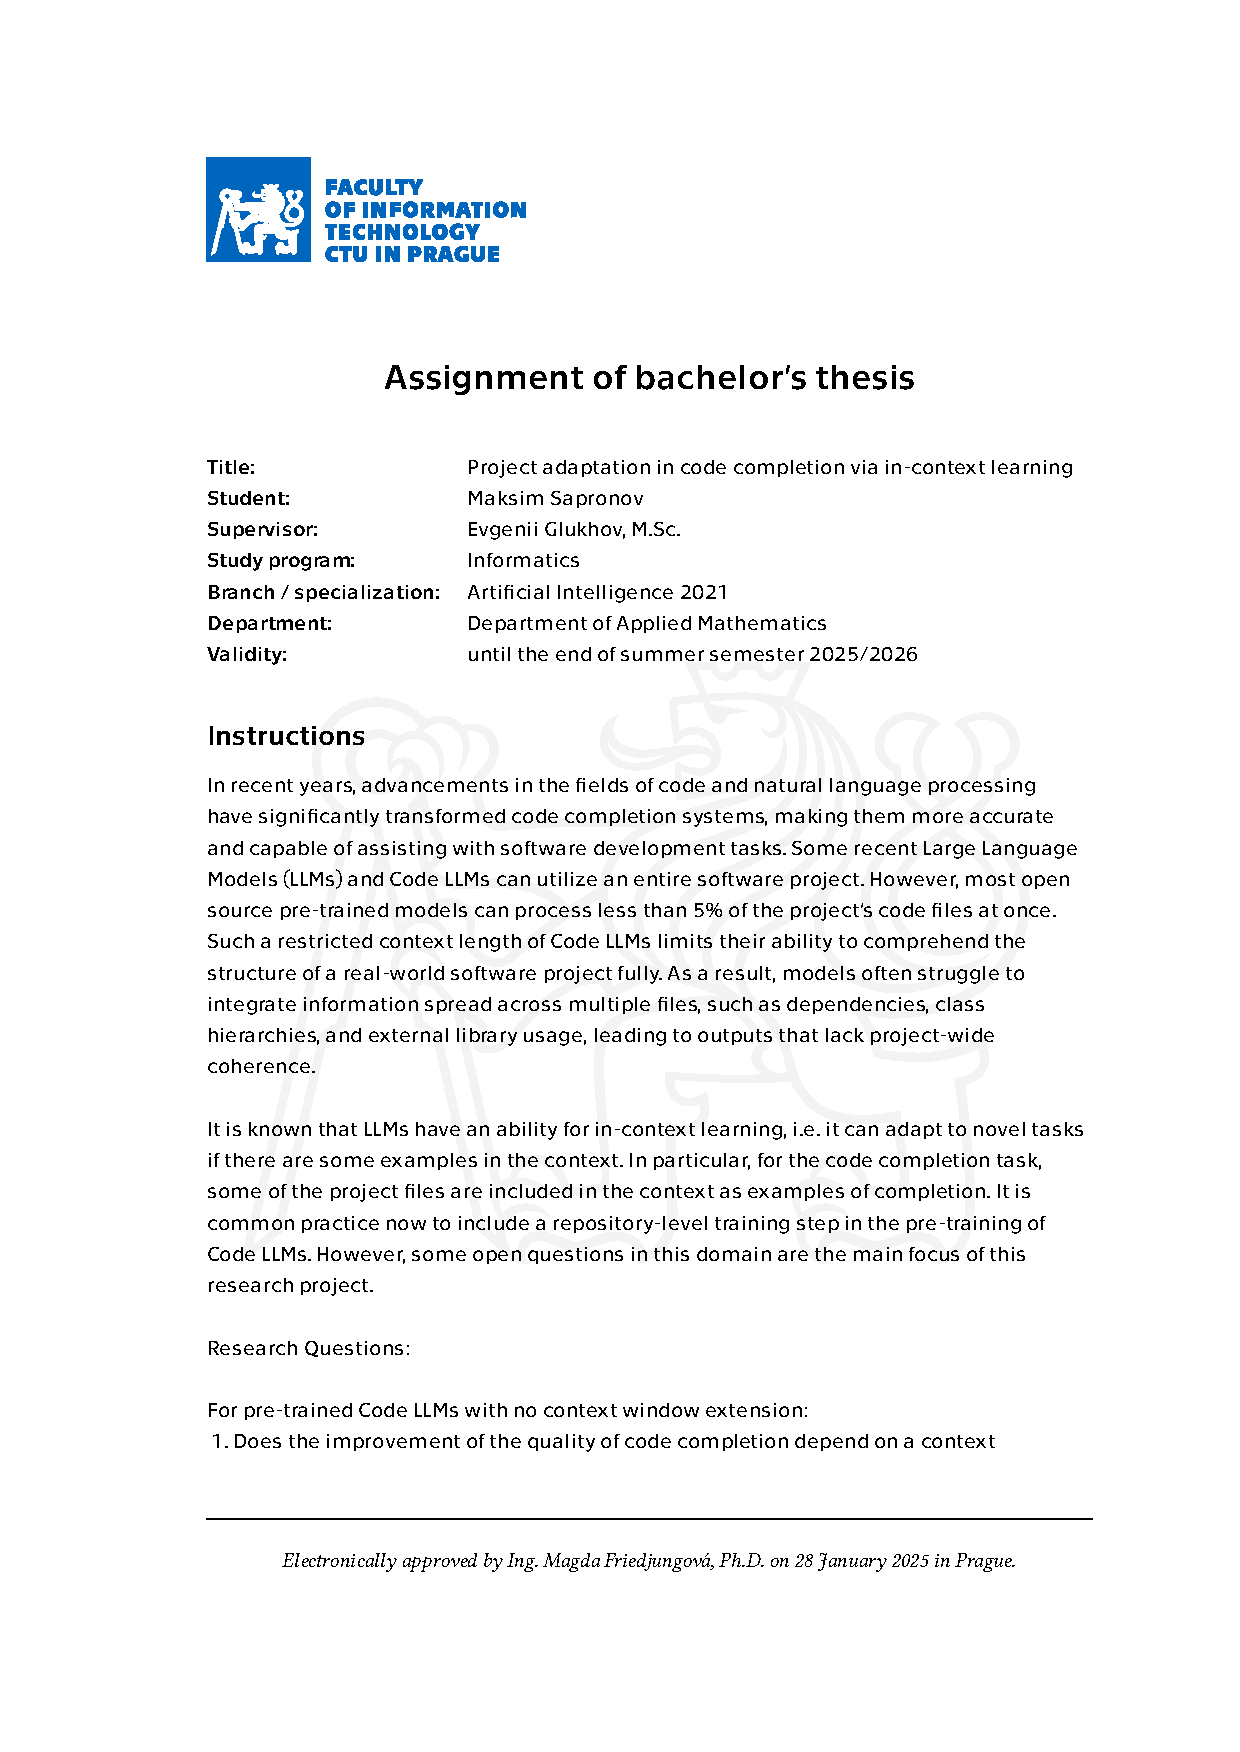
\includepdf[pages={1-}]{assignment.pdf}

\imprintpage
\stopTOCentries
%%%%%%%%%%%%%%%%%%%%%%
% list of other contents END
%%%%%%%%%%%%%%%%%%%%%%

% TODO: fill in the acknowledgment page
\begin{acknowledgmentpage}
	Thank you $\dots$
\end{acknowledgmentpage}

% TODO: choose one of approved texts of the declaration. DO NOT CREATE YOUR OWN. Find the approved texts at https://courses.fit.cvut.cz/SFE/download/index.html#_documents (document Declaration for FT in English)
\begin{declarationpage}
    Declaration content.
\end{declarationpage}

\printabstractpage

% TODO: decide whether to include the summary

\tableofcontents
%%%%%%%%%%%%%%%%%%%%%%
% list of other contents: figures, tables, code listings, algorithms, etc.
% add/remove commands accordingly
%%%%%%%%%%%%%%%%%%%%%%
\listoffigures % list of figures
\begingroup
\let\clearpage\relax
\listoftables % list of tables
\thectufitlistingscommand
\endgroup

% TODO: fill in the abbreviations (here is an irrelevant example)
\chapter{\thectufitabbreviationlabel}

\begin{tabular}{rl}
DFA & Deterministic Finite Automaton\\
FA & Finite Automaton\\
LPS & Labelled Prüfer Sequence\\
NFA & Nondeterministic Finite Automaton\\
NPS & Numbered Prüfer Sequence\\
XML & Extensible Markup Language\\
XPath & XML Path Language\\
XSLT & eXtensible Stylesheet Language Transformations\\
W3C & World Wide Web Consortium
\end{tabular}

\resumeTOCentries
\mainmatter\mainmatterinit
%%%%%%%%%%%%%%%%%%%
% THE THESIS
% MODIFY ANYTHING BELOW THIS LINE
%%%%%%%%%%%%%%%%%%%

\chapter*{Objectives of the Thesis}\addcontentsline{toc}{chapter}{Objectives of the Thesis}\markboth{Objectives of the Thesis}{Objectives of the Thesis}

The objectives of this thesis are divided into two parts, corresponding to the theoretical and practical aspects of the work.

The theoretical part aims to provide a comprehensive survey of the challenges associated with project adaptation in the context of full line code completion, focusing on the current capabilities and limitations of in-context learning and repository-level code completion methods. This part establishes the necessary background to understand the practical contributions of the thesis.

The practical part addresses several research questions concerning the impact of various context composition strategies on the quality of code completion, evaluated across three setups: a pre-trained Code Large Language Model (Code LLM), the same model fine-tuned with a specific context composition strategy, and the model after context window extension. To address these questions, the thesis implements a context composition framework for extracting relevant information from software repositories, as well as a fine-tuning pipeline for adapting Code LLMs to project-specific data. The outcomes characterize the role of context composition in enhancing code completion quality and provide insights into its integration within repository-level training procedures.

\chapter*{Introduction}\addcontentsline{toc}{chapter}{Introduction}\markboth{Introduction}{Introduction}

Software development plays a pivotal role in shaping the modern digital world. Assisting developers in writing code more efficiently has the potential to accelerate innovation across industries by reducing the cognitive and temporal overhead of programming. Over the decades, numerous tools have emerged to support developers, including high-level programming languages, integrated development environments (IDEs), version control systems, and, more recently, AI-powered code assistance. Tasks such as code completion, generation, refactoring, and bug localization are increasingly addressed using Large Language Models (LLMs), which have demonstrated strong capabilities in natural language and code understanding.

Code completion, in particular, benefits significantly from the in-context learning capabilities of LLMs — where the model leverages examples or relevant information provided in the input context to improve predictions without parameter updates. However, while LLMs have advanced in modeling local contexts, a critical limitation remains: their restricted ability to integrate and reason over information dispersed across large codebases. This includes understanding dependencies between files, class hierarchies, and interactions with external libraries — information that is often essential for generating coherent and accurate completions.

Despite the emergence of code-specific LLMs and efforts to incorporate repository-level context during training or inference, most pre-trained models still struggle to process more than a small fraction of a project's code files at once. As a result, they fall short in capturing project-wide structure, leading to incomplete or inaccurate predictions. Therefore, there is a need for continued research within the community developing such models to address these limitations. This thesis focuses on exploring how the composition and organization of contextual information influence the performance of code completion models, particularly in repository-level settings where code is distributed across multiple interdependent files. It investigates how context selection strategies and model adaptations can enhance the ability of pre-trained Code LLMs to generate coherent and accurate completions that reflect the structure and semantics of entire software projects.

% TODO: highlight the novelty of the work
% TODO: references?
% TODO: fill in the structure of the thesis here (w/ or w/o the example list)
% \begin{description}
    % \item[Chapter 1] Description of the first chapter.
    % \item[Chapter 2] Description of the second chapter.
% \end{description}


\appendix\appendixinit

\chapter{Appendix}

\section{Supplementary Figures and Tables}

\begin{table}[htbp]
    \centering
    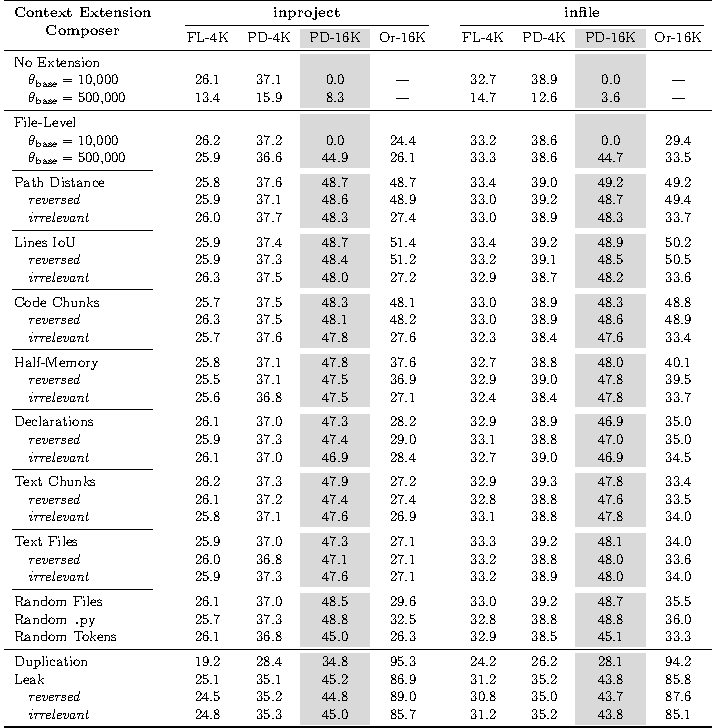
\includegraphics[width=\textwidth]{tables/rq-b.pdf}
    \caption{Extended table presenting the evaluation results for OpenCoder-1.5B-Base, which underwent the repository-level pre-training stage. A more detailed description of the evaluation setup is provided in Section~\ref{sec:evaluation}.}\label{tab:ocoder-extension-extended}
\end{table}

\begin{table}[htbp]
    \centering
    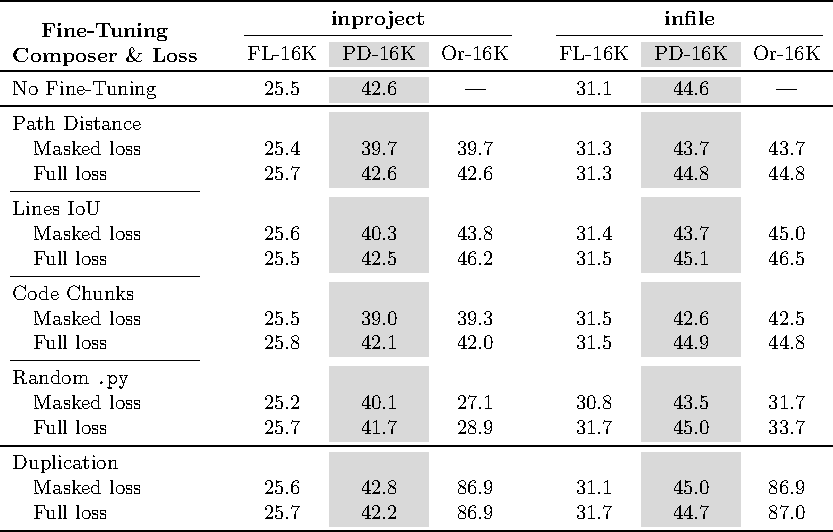
\includegraphics[width=\textwidth]{tables/rq-a2-gradient-masking.pdf}
    \caption{Exact Match scores for DeepSeek-Coder-Base 1.3B fine-tuned on composers generating inlier repository context for the completion file under two training setups: with and without gradient masking}\label{tab:dseek-gradient-masking}
\end{table}

\begin{table}[htbp]
    \centering
    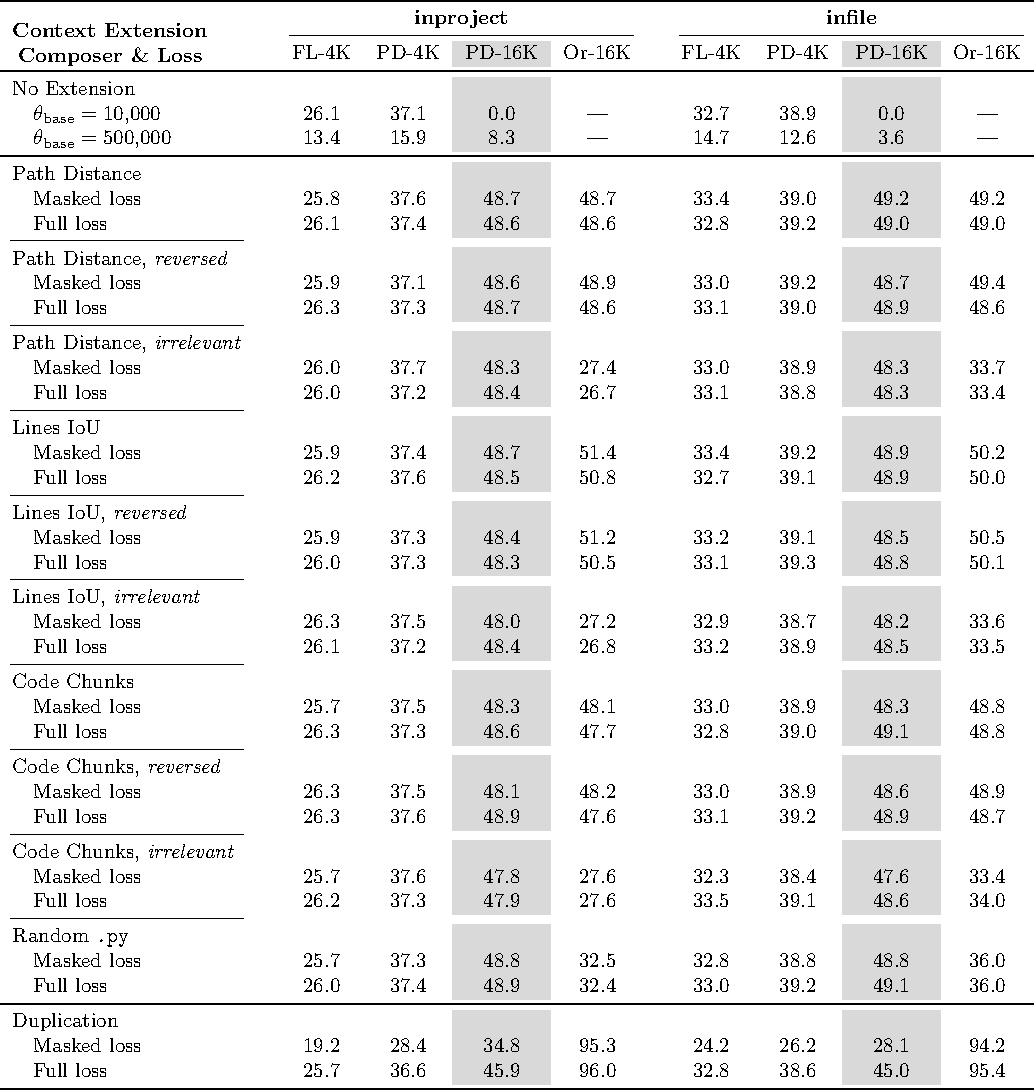
\includegraphics[width=\textwidth]{tables/rq-b-gradient-masking.pdf}
    \caption{Exact Match scores for repository-level pre-trained OpenCoder-1.5B-Base on composers generating inlier repository context for the completion file under two training setups: with and without gradient masking}\label{tab:ocoder-gradient-masking}
\end{table}

\begin{figure}[ht]
    \centering
    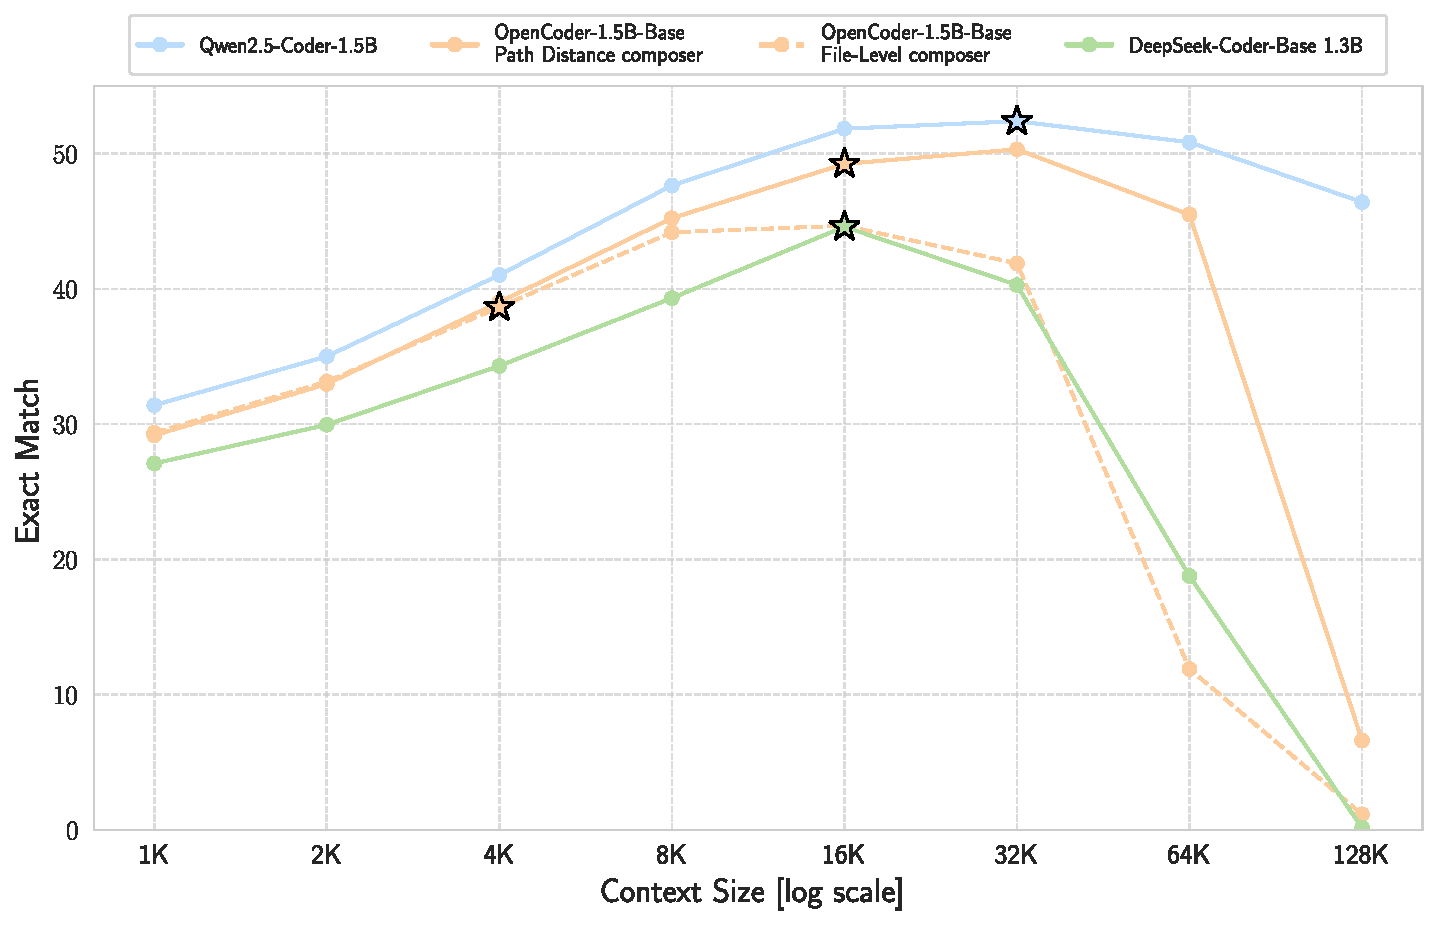
\includegraphics[width=\textwidth]{figures/beyond-training-window-infile.pdf}
    \caption{Evaluation of the performance scaling beyond the context extension window. The \textit{infile} line type from the LCA benchmark is selected for visualization; the corresponding Figure~\ref{fig:beyond-training-window-inproject} presents results for the \textit{inproject} category. ``1K'' refers to 1,024 tokens. The \raisebox{-0.3ex}{\FiveStarOpen} markers denote the context length used during repository-level pre-training stage.}\label{fig:beyond-training-window-infile}
\end{figure}
 % include `appendix.tex' from `text/' subdirectory

\backmatter

\printbibliography % print out the BibLaTeX-generated bibliography list

\chapter{Contents of the attachment}

Not ready.

	% TODO: fill in the contents of the attachment (irrelevant example is provided)
	% \dirtree{%
	% 	.1 /.
	% 	.2 readme.txt\DTcomment{short description of the media}.
	% 	.2 exe\DTcomment{directory with the executable form of the implementation}.
	% 	.2 src.
	% 	.3 impl\DTcomment{source codes of the implementation}.
	% 		.3 thesis\DTcomment{zdrojová forma práce ve formátu \LaTeX{}}.
	% 		.2 text\DTcomment{text práce}.
	% 		.3 thesis.pdf\DTcomment{text práce ve formátu PDF}.
	% }
 % include `medium.tex' from `text/' subdirectory

\end{document}
